\documentclass[12pt]{article}
\usepackage[left=1cm, right=1cm, top=2cm,bottom=1.5cm]{geometry} 

\usepackage[parfill]{parskip}
\usepackage[utf8]{inputenc}
\usepackage[T2A]{fontenc}
\usepackage[russian]{babel}
\usepackage{enumitem}
\usepackage[normalem]{ulem}
\usepackage{amsfonts, amsmath, amsthm, amssymb, mathtools}

\usepackage{fancyhdr}
\pagestyle{fancy}
\renewcommand{\headrulewidth}{1.5pt}
\renewcommand{\footrulewidth}{1pt}

\usepackage{graphicx}
\usepackage[figurename=Рис.]{caption}
\usepackage{subcaption}
\usepackage{float}

%%Наименование папки откуда забирать изображения
\graphicspath{ {./images/} }

%%Изменение формата для ввода доказательства
\renewcommand{\proofname}{$\square$  \nopunct}
\renewcommand\qedsymbol{$\blacksquare$}

\addto\captionsrussian{%
	\renewcommand{\proofname}{$\square$ \nopunct}%
}
%% Римские цифры
\newcommand{\RN}[1]{%
	\textup{\uppercase\expandafter{\romannumeral#1}}%
}

%% Для удобства записи
\newcommand{\MR}{\mathbb{R}}
\newcommand{\MQ}{\mathbb{Q}}
\newcommand{\MI}{\mathrm{I}}
\newcommand{\MJ}{\mathrm{J}}
\newcommand{\MH}{\mathrm{H}}
\newcommand{\MU}{\mathcal{U}}
\newcommand{\MV}{\mathcal{V}}
\newcommand{\VN}{\varnothing}
\newcommand{\VE}{\varepsilon}

\theoremstyle{definition}
\newtheorem{defn}{Опр:}
\newtheorem{rem}{Rm:}
\newtheorem{prop}{Утв.}
\newtheorem{exrc}{Упр.}
\newtheorem{lemma}{Лемма}
\newtheorem{theorem}{Теорема}
\newtheorem{corollary}{Следствие}

\newenvironment{cusdefn}[1]
{\renewcommand\thedefn{#1}\defn}
{\enddefn}

\DeclareRobustCommand{\divby}{%
	\mathrel{\text{\vbox{\baselineskip.65ex\lineskiplimit0pt\hbox{.}\hbox{.}\hbox{.}}}}%
}
%Коротки минус
\DeclareMathSymbol{\SMN}{\mathbin}{AMSa}{"39}

\newcommand{\smallerrel}[1]{\mathrel{\mathpalette\smallerrelaux{#1}}}
\newcommand{\smallerrelaux}[2]{\raisebox{.1ex}{\scalebox{.75}{$#1#2$}}}

\newcommand{\smallin}{\smallerrel{\in}}
\newcommand{\smallnotin}{\smallerrel{\notin}}

\newcommand*{\medcap}{\mathbin{\scalebox{1.25}{\ensuremath{\cap}}}}%
\newcommand*{\medcup}{\mathbin{\scalebox{1.25}{\ensuremath{\cup}}}}%

\begin{document}
\lhead{Математический анализ - I}
\chead{Шапошников С.В.}
\rhead{Лекция - 23}

\section*{Правила дифференцирования}

\subsection*{Дифференциал композиции функций}
\begin{theorem}\textbf{(Дифф. сложной функции)}
	Пусть $f$ - дифференцируема в точке $a$, $g$ - дифференцируема в точке $f(a)$. Тогда $g(f(x))$ - дифференцируема в точке $a$ и $$\big( g(f(x))\big)^\prime(a) = g^\prime(f(a)){\cdot}f^\prime(a)$$
\end{theorem}

Перепишем этот результат в терминах дифференциала (по определению $=$ производная$\cdot h$): 
$$d(g\circ f)(h) = g^\prime\big(f(a) \big)\underbrace{f^\prime(a){\cdot}h}_{=df(h)} = g^\prime\big(f(a) \big)df(h) = dg(df(h))$$ 
где $df(h)$ это результат действия линейной функции $df$ на приращение $h$, который в свою очередь также можно трактовать как приращение $\Rightarrow dg(df(h))$ это результат действия линейной функции $dg$ на приращение $df(h)$. 
\begin{rem}
	Полезно трактовать $h$ как вектор перемещения для аргумента функции $\Rightarrow$ взяли вектор $h$, применили линейную функцию, получили вектор $f(h)$ и подставили этот вектор в дифференциал функции $g \Rightarrow$ поэтому верно всегда
	$$d(g \circ f) = dg \circ df$$
\end{rem}

Данный результат согласуется с нашим пониманием дифференциала, как линейной функции:\\
$dg(t) = g^\prime(f(a))t \Leftrightarrow z = k_1{\cdot}t$ - линейная функция. $df(h) = f^\prime(a){\cdot}h \Leftrightarrow t = k_2{\cdot}h$ - линейная функция. Композиция этих двух линейных функций $z = k_1(k_2h) = (k_1k_2)h$ - линейная функция, коэффициент которой равен произведению коэффициентов линейных функций, которые брали до этого. 

\subsection*{Инвариантность $\RN{1}$-го дифференциала}

Рассмотрим запись
$$dg(f(x)) = g^\prime(f(x))df \Rightarrow dg(f) = g^\prime(f)df$$ 
Дописав $x$ получим правило дифференцирования сложной функции. Тогда
\begin{enumerate}
	\item если считать, что $f$ это переменная, то мы получим здесь определение дифференциала. 
	\item если считать, что $f$ это функция - это также верно. 
\end{enumerate}

То есть в этой записи не важно, считаем $f$ функцией или свободной переменной. Это называется \uwave{инвариантностью $\RN{1}$-го дифференциала}, что его вид не зависит от трактования $f$.

Пусть $\MR_x \xrightarrow{f} \MR_y$, функция $g(y)$ определена на $\MR_y \Rightarrow$ возникает новая функция $g(y) \rightarrow g(f(x))$ которая определена на $\MR_x \Rightarrow$ поменяли систему координат. Если бы $f$ была взаимно-однозначной, эта была бы честная замена координат. 

Пусть все функции дифференцируемы и у $g(y)$ дифференциал был бы равен $dg = g^\prime(y)dy$. Оказывается, что для новой функции вместо $y$ надо просто подставить $f \Rightarrow dg(f) = g^\prime(f)df \Rightarrow$ форма дифференциала остается неизменной, то есть его вид не зависит от замены координат.

\begin{rem}
	Для дифференциалов более высоких порядков это совершенно не так.
\end{rem}

\uline{\textbf{Инвариантность $\RN{1}$-го дифференицала}}: Вид дифференциала не зависит от выбора системы координат или в равенстве $dg = g^\prime(y)dy, \, y$ можно считать свободной переменной или функцией и ответ в любом случае правильный. 

\subsection*{Дифференцирование обратной функции}

\begin{theorem} \textbf{(О существовании обратной функции)}
	Пусть $f$ непрерывна и строго монотонна на промежутке $\MI$. Тогда $f(\MI)$ - промежуток и определена обратная функция $f^{-1}\colon f(\MI) \to \MI$, причем $f^{-1}$ строго монотонна и непрерывна.
\end{theorem}

\begin{prop}
	Если $f$ дифференцируема в точке $a \in \MI$ - внутренняя точка промежутка $\MI$ и $f^\prime(a) \neq 0$, то $f^{-1}$ дифференцируема в точке $f(a)$ - внутренняя точка промежутка $f(I)$ и $$(f^{-1})^\prime(f(a)) = \dfrac{1}{f^\prime(a)} \vee d(f^{-1})(h) = \dfrac{1}{f^\prime(a)}{\cdot}h$$
\end{prop}

\begin{rem}
	Дифференциал функции $f, \, df(h) = f^\prime(a){\cdot}h$, то есть линейная функция $y = kx \Rightarrow$ обратная функция к ней $x = \frac{1}{k}y \Rightarrow$ дифференциал обратной функции это обратная функция к дифференциалу $\Rightarrow df^{-1} = (df)^{-1}$
\end{rem}

\begin{rem}
	Доказательство будет проще, чем в случае со сложными функциями, так как $f$ это биекция этих промежутков. Поэтому никогда не может случиться, что при $x\neq a \Rightarrow f(x) = f(a)$.
\end{rem}

\begin{proof}
	$\lim\limits_{y \to f(a)}\dfrac{f^{-1}(y) - f^{-1}(f(a))}{y-a} = \lim\limits_{y \to f(a)}\MH(f^{-1}(y))$, где $\MH(x) = \dfrac{x-a}{f(x) - f(a)}$. Про функцию $\MH(x)$ мы знаем, что $\lim\limits_{x \to a}\MH(x) = \frac{1}{f^\prime(a)}$ по определению.
	С другой стороны, мы знаем, что $\lim\limits_{y \to f(a)}f^{-1}(y) = a$ из-за непрерывности функции $f^{-1}$. Так как $f$ биекция, то $f^{-1}(y) \neq a$ при $y \neq f(a) \Rightarrow$ по теореме о пределе композиций: $$\lim\limits_{y \to f(a)}\dfrac{f^{-1}(y) - f^{-1}(f(a))}{y-a} = \lim\limits_{y \to f(a)}\MH(f^{-1}(y)) = \dfrac{1}{f^\prime(a)}$$
\end{proof}

\begin{rem}
	Другая запись теоремы о производной обратной функции $(f(a) = b)$:
	$$(f^{-1})^\prime(b) =\frac{1}{f^\prime(f^{-1}(b))}$$
\end{rem}

Перед тем, как составлять таблицу производных, вспомним замечательные пределы:
\begin{lemma}\hfill
	\begin{enumerate}[label={\arabic*)}]
		\item $\lim\limits_{x \to 0}\dfrac{\ln(1+x)}{x} =1$;
		\item $\lim\limits_{x \to 0}\dfrac{e^x - 1}{x} = 1$;
	\end{enumerate}
\end{lemma}
\begin{proof}\hfill
		\begin{enumerate}[label={\arabic*)}]
		\item $\lim\limits_{x \to 0}\dfrac{\ln(1+x)}{x} \underset{x = \frac{1}{t}}{=} \lim\limits_{t \to \infty}\dfrac{\ln(1+\frac{1}{t})}{\frac{1}{t}} = \lim\limits_{t \to \infty}\ln(1+\frac{1}{t})^t \Rightarrow$ по непрерывности $\ln{x} \Rightarrow  \lim\limits_{t \to \infty}\ln(1+\frac{1}{t})^t = \ln{e} = 1$;
		\item Так как $e^x$ - непрерывна и $x \to 0 \Rightarrow e^x - 1 \to 1-1 = 0 \Rightarrow\lim\limits_{x \to 0}\dfrac{e^x - 1}{x} \underset{e^x -1 = t}{=} \lim\limits_{t \to 0}\dfrac{t}{\ln{(1+t)}}=1$;
	\end{enumerate}
\end{proof}

\newpage

\section*{Таблица производных}
\begin{enumerate}[label={(\arabic*)}]
	\item $(\text{const})^\prime = 0$;
		\begin{proof}
			$\lim\limits_{x \to a}\dfrac{c - c}{x-a} = 0$, где $c = \text{const}$;
		\end{proof}
	\item $(x^n)^\prime = nx^{n-1}$, где $x \in \MR, \, n \in \mathbb{N} \vee x \neq 0, \, n \in \mathbb{Z}$;
		\begin{proof}
			$\lim\limits_{x \to a}\dfrac{x^n - a^n}{x-a} =\lim\limits_{x \to a}\dfrac{(x-a)(x^{n-1} + ax^{n-2}+ \dotsc + a^{n-1})}{x-a} = \lim\limits_{x \to a}(x^{n-1} + ax^{n-2}+ \dotsc + a^{n-1}) = na^{n-1}$;
		\end{proof}
	\item $(e^x)^\prime = e^x$;
		\begin{proof}
			$\lim\limits_{x \to a}\dfrac{e^x - e^a}{x-a} =e^a\lim\limits_{x \to a}\dfrac{e^{(x-a)} - 1}{(x-a)} = e^a$;
		\end{proof}
	\item $(\ln{x})^\prime = \dfrac{1}{x}$;
		\begin{proof}
			Хотим найти производную функции $\ln{x}$ в точке $x = a$, тогда обратная фуннкция в этой точке $e^y = a \Rightarrow y = \ln{a} \Rightarrow$ по теореме о дифференцировании обратной функции $\Rightarrow$
			$$ (\ln{x})^\prime(a) =\dfrac{1}{(e^y)^\prime(\ln{a})} = \dfrac{1}{a}$$
		\end{proof}
\end{enumerate}

\begin{corollary}
	$x > 0, \, \alpha \in \MR \Rightarrow (x^\alpha) = \alpha x^{\alpha-1}$.
\end{corollary}
\begin{proof}
	$x^\alpha = e^{\alpha \ln{x}} \Rightarrow$ дифференцируем как сложную функцию $$ (x^\alpha)^\prime = e^{\alpha \ln{x}}{\cdot}(\alpha \ln{x})^\prime =  e^{\alpha \ln{x}}{\cdot}\dfrac{\alpha}{x} = x^\alpha{\cdot}\dfrac{\alpha}{x} = \alpha x^{\alpha-1}$$
\end{proof}
\begin{exrc}
	Доказать, что функция $\cos{x}$ - непрерывная функция.
\end{exrc}
\begin{enumerate}[label={(\arabic*)}]
	\setcounter{enumi}{4}
	\item $(\sin{x})^\prime = \cos{x}, \, (\cos{x})^\prime = -\sin{x}$;
		\begin{proof}
			$\lim\limits_{x \to a}\dfrac{\sin{x} - \sin{a}}{x-a} = \lim\limits_{x \to a}\dfrac{\sin{\tfrac{x-a}{2}}\cos{\tfrac{x+a}{2}}}{\tfrac{x-a}{2}} = \lim\limits_{x \to a}\dfrac{\sin{\tfrac{x-a}{2}}}{\tfrac{x-a}{2}}{\cdot}\cos{\tfrac{x+a}{2}} = \cos{a}$;
			
			$(\cos{x})^\prime = (\sin{(\frac{\pi}{2}-x)})^\prime = \cos{(\frac{\pi}{2}-x)}{\cdot}(-1) = - \sin{x}$;
		\end{proof}
	\item $(\tg{x})^\prime = \dfrac{1}{\cos^2{x}}, \, (\ctg{x})^\prime = -\dfrac{1}{\sin^2{x} };$
		\begin{proof}
			Используем правило Лейбница $\Rightarrow$ 
			$$ \Rightarrow (\tg{x})^\prime = \Big(\frac{\sin{x}}{\cos{x}} \Big)^\prime = \frac{\cos{x}}{\cos{x}} + \sin{x}{\cdot} \Big(\frac{1}{\cos{x}} \Big)^\prime = 1 + \sin{x}{\cdot}\Big(\frac{\sin{x}}{\cos^2{x}}\Big) = 1 + \tg^2{x} = \dfrac{1}{\cos^2{x} }$$
			$$ \Rightarrow (\ctg{x})^\prime = \Big(\frac{\cos{x}}{\sin{x}} \Big)^\prime = -\frac{\sin{x}}{\sin{x}} + \cos{x}{\cdot} \Big(\frac{1}{\sin{x}} \Big)^\prime = -1 - \cos{x}{\cdot}\Big(\frac{\cos{x}}{\sin^2{x}}\Big) = -1 - \ctg^2{x} = -\dfrac{1}{\sin^2{x} }$$
		\end{proof}
	\newpage
	\item $(\arcsin{x})^\prime = \dfrac{1}{\sqrt{1-x^2}}, \, (\arccos{x})^\prime = -\dfrac{1}{\sqrt{1-x^2}}$;
		\begin{proof}
			$$(\arcsin{x})^\prime = \dfrac{1}{(\sin{y})^\prime}\Big|_{y = \arcsin{x}} = \dfrac{1}{\cos{(\arcsin{x})}} = \dfrac{1}{\pm \sqrt{1 - \sin^2{(\arcsin{x})}} } = \dfrac{1}{\pm\sqrt{1 - x^2}}$$ 
			Поскольку $\arcsin{x}$ определен на $(-\tfrac{\pi}{2},\tfrac{\pi}{2})$, то $\cos{x} \geq 0, \forall x\in (-\tfrac{\pi}{2},\tfrac{\pi}{2}) \Rightarrow (\arcsin{x})^\prime = \dfrac{1}{\sqrt{1 - x^2}}$.\\
			Поскольку $\arcsin{x} + \arccos{x} = \frac{\pi}{2} \Rightarrow (\arccos{x})^\prime = (\frac{\pi}{2} - \arcsin{x})^\prime = - \dfrac{1}{\sqrt{1-x^2}}$.
		\end{proof}
	\item $(\arctg{x})^\prime = \dfrac{1}{1 + x^2}, \, (\arcctg{x})^\prime = -\dfrac{1}{1 + x^2}$;
		\begin{proof}
			$$(\arctg{x})^\prime = \dfrac{1}{(\tg{y})}\Big|_{y = arctg{x}} = \dfrac{1}{1 + \tg^2{(\arctg{x})}} = \dfrac{1}{1 + x^2}$$
			Поскольку $\arctg{x} + \arcctg{x} = \frac{\pi}{2} \Rightarrow (\arcctg{x})^\prime = (\frac{\pi}{2} - \arctg{x})^\prime = - \dfrac{1}{1+ x^2}$.
		\end{proof}
	\item $(\ch{x})^\prime = \Big(\dfrac{e^x + e^{-x}}{2}\Big)^\prime = \sh{x}, \, (\sh{x})^\prime = \Big(\dfrac{e^x - e^{-x}}{2}\Big)^\prime = \ch{x}, \, (\th{x})^\prime = \dfrac{1}{\ch^2{x}}$;
		\begin{proof}
			$$(\ch{x})^\prime = \Big(\dfrac{e^x + e^{-x}}{2}\Big)^\prime = \Big(\dfrac{e^x - e^{-x}}{2}\Big) = \sh{x}, \, (\sh{x})^\prime = \Big(\dfrac{e^x - e^{-x}}{2}\Big)^\prime = \Big(\dfrac{e^x + e^{-x}}{2}\Big) = \ch{x}$$
			Воспользуемся правилом Лейбница 
			$$(\th{x})^\prime =  \Big(\dfrac{e^x - e^{-x}}{e^x + e^{-x}}\Big)^\prime = \dfrac{e^x + e^{-x}}{e^x + e^{-x}} + (e^x - e^{-x}){\cdot}\Big( \dfrac{1}{e^x + e^{-x}}\Big)^\prime = 1 + (e^x - e^{-x}){\cdot}\dfrac{e^x - e^{-x}}{(e^x + e^{-x})^2} = 1 + \th^2{x} = \dfrac{1}{\ch^2{x}}$$
		\end{proof}
\end{enumerate}

\newpage
\section*{Основные теоремы дифференциального исчисления}
\begin{theorem}\textbf{(Ферма)}
	Пусть $f$ определена в окрестности $\MU(a)$ точки $a$ и $\forall x \in \MU(a), \, f(x) \leq f(a)$ (или $\forall x \in \MU(a), \, f(x) \geq f(a)$). Если $f$ дифференцируема в точке $a$, то $f^\prime(a) = 0$.
\end{theorem}

\begin{figure}[H]
	\centering
	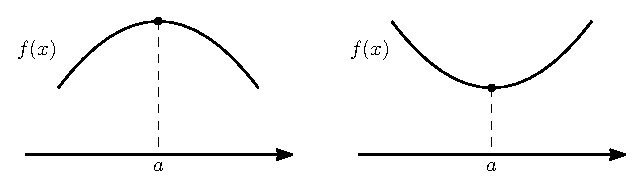
\includegraphics[width=0.55\textwidth]{23_1.eps}
	\caption{$\forall x \in \MU(a), \, f(x) \leq f(a) \vee f(x) \geq f(a)$.}
	\label{23_1}
\end{figure}

\begin{proof}
	Пусть $\forall x \in \MU(a), \, f(x) \geq f(a) \Rightarrow f(x) - f(a) \geq 0$, тогда рассмотрим следующие пределы 
	$$\lim\limits_{x \to a+}\dfrac{f(x) - f(a)}{x-a} \geq 0, \, \lim\limits_{x \to a-}\dfrac{f(x) - f(a)}{x-a} \leq 0$$
	Поскольку $f$ дифференцируема в точке $a \Rightarrow f$ неперерывна в точке $a \Rightarrow$
	$$ \Rightarrow 0 \leq \lim\limits_{x \to a+}\dfrac{f(x) - f(a)}{x-a} = f^\prime(a) = \lim\limits_{x \to a-}\dfrac{f(x) - f(a)}{x-a} \leq 0 \Rightarrow f^\prime(a)   = 0$$
\end{proof}
\uline{\textbf{Геометрический смысл теоремы Ферма}}: $f^\prime(a) = 0$ означает, что касательная в точке $(a,f(a))$ паралелльна оси $x$.
\begin{figure}[H]
	\centering
	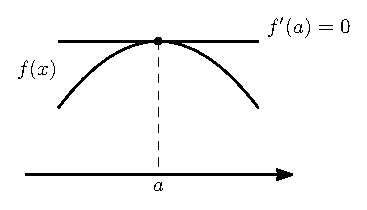
\includegraphics[width=0.35\textwidth]{23_2.eps}
	\caption{Геометрический смысл теоремы Ферма.}
	\label{23_2}
\end{figure}
\uline{\textbf{Физический смысл теоремы Ферма}}: По прямой двигается точка, её координата $x$ меняется со временем $x(t)$ (меняется так, что скорость есть, в каждой точке $t$ дифференцируема). Тогда в момент времени $t = a$ мы находимся на максимальном удалении. Дальше мы будем находится к началу движения ближе или не дальше.

\begin{theorem}\textbf{(Ролль)}
	Пусть $f$ непрерывна на отрезке $[a,b]$ и дифференцируема на интервале $(a,b)$. Если $f(a) = f(b)$, то $\exists \, c \in (a,b) \colon f^\prime(c) = 0$.
\end{theorem}
\uline{\textbf{Геометрический смысл теоремы Ролля}}: Если значения на концах отрезка равны, обязательно в какой-то момент касательная обязана быть параллельной оси $x$.

\uline{\textbf{Физический смысл теоремы Ферма}}: Если вы вернулись туда же, откуда выехали по прямой, то обязательно был момент, когда вы остановились (перемещение нулевое, значит был момент, когда мгновенная скорость тоже была нулевой).

\begin{figure}[H]
	\centering
	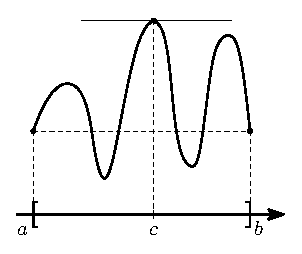
\includegraphics[width=0.25\textwidth]{23_3.eps}
	\caption{Геометрический смысл теоремы Ролля.}
	\label{23_3}
\end{figure}

\begin{proof}
	Функция $f$ непрерывна на отрезке, тогда по теореме Вейрштрасса 
	$$\exists \, x_m, x_M \in [a,b] \colon f(x_m) = \min\limits_{[a,b]}{f}, f(x_M) = \max\limits_{[a,b]}{f}$$
	Если хотя бы одна из этих точек $x_m$ и $x_M$ лежит внутри интервала $(a,b)$, то по теореме Ферма в этой точке производная $= 0$. Если $x_m$ и $x_M$ совпадают с $a$ или $b$, то $\min\limits_{[a,b]}{f} = \max\limits_{[a,b]}{f} \Rightarrow f = \text{const} \Rightarrow c$ - любая точка интервала.
\end{proof}

\begin{theorem}\textbf{(Лагранжа о среднем)}
	Пусть $f$ непрерывна на отрезке $[a,b]$ и дифференцируема на интервале $(a,b)$. Тогда $\exists \, c \in (a,b) \colon f(b) - f(a) = f^\prime(c)(b-a)$ или аналогично
	$$\exists \, c \in (a,b) \colon \dfrac{f(b) - f(a)}{b-a} = f^\prime(c)$$
\end{theorem}
\uline{\textbf{Геометрический смысл теоремы Лагранжа}}: существует точка $c$ на интервале $(a,b)$ в которой касательная функции $f$ параллельна её хорде на отрезке.
\begin{figure}[H]
	\centering
	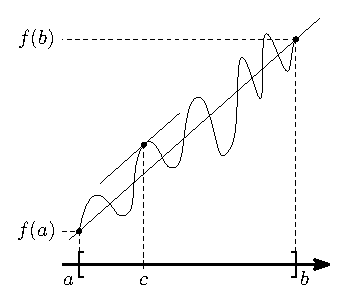
\includegraphics[width=0.3\textwidth]{23_4.eps}
	\caption{Геометрический смысл теоремы Лагранжа: $\tfrac{f(b) - f(a)}{b-a}$ - наклон хорды и $f^\prime(c)$ - наклон касательной совпадают в точе $c$. \uline{Уравнение хорды}: $\tfrac{f(b)-f(a)}{b-a}(x-a) + f(a)$.}
	\label{23_4}
\end{figure}
\uline{\textbf{Физический смысл теоремы Лагранжа}}: $\tfrac{f(b) - f(a)}{b-a}$ - средняя скорость, $f^\prime(c)$ - мгновенная скорость $\Rightarrow$ есть точка, где мгновенная скорость совпадала со средней.
\begin{proof}
	Возьмем $F(x) = f(x) - \Big(\tfrac{f(b)-f(a)}{b-a}(x-a) + f(a) \Big ) \Rightarrow F(b) = F(a) = 0 \Rightarrow$ применяем теорему Ролля $\Rightarrow \exists \, c \in(a,b) \colon F^\prime(c) = 0 \Rightarrow F^\prime(c) = f^\prime(c) - \dfrac{f(b)-f(a)}{b-a} = 0 \Rightarrow f^\prime(c) = \dfrac{f(b)-f(a)}{b-a}$.
\end{proof}

\end{document}